%!TEX root = ./template-skripsi.tex
%-------------------------------------------------------------------------------
%                            BAB II
%               TINJAUAN PUSTAKA DAN DASAR TEORI
%-------------------------------------------------------------------------------


\chapter{TINJAUAN PUSTAKA DAN DASAR TEORI}                

\section{Tinjauan Pustaka}
\indent Penelitian mengenai karakterisasi aspek afektif yang timbul karena sentuhan (tactile) sebelumnya telah banyak dilakukan. Berbagai pendekatan banyak digunakan untuk memetakan aspek afektif dari sentuhan dalam suatu fenomena atau besaran yang terukur. Salah satu metode yang banyak digunakan adalah fMRI (functional magnetic resonance imaging) untuk mengetahui bagian otak yang bereaksi saat sentuhan yang menimbulkan afeksi timbul. Dalam penelitian yang dilaksanakan oleh Ilanit Gordon dkk menyatakan bahwa bagian otak yang bereaksi ketika sentuhan afektif terjadi adalah daerah di sekitar amigdala dan insula \cite{Gordon2013}⁠. Penelitian serupa juga dilakukan untuk mengetahui bagian tubuh manusia yang paling peka untuk menimbulkan respon afektif. Dari fMRI diketahui bahwa bagian tubuh yang memiliki bulu lebih peka untuk menimbulkan respon afektif \cite{Mcglone2012}⁠.\\ 
\indent Selain fMRI banyak penelitian lain yang dilakukan untuk karakterisasi respon afektif  menggunakan metode statistik. Pada umumnya metode ini digunakan untuk mengetahui dimensi dari respon afektif serta pengelompokkan respon afektif yang timbul dari sentuhan. Terdapat lima dimensi pada sentuhan yaitu kekasaran makro dan murni, hangat/dingin, keras/lembut, dan gesekan \cite{Okamoto2013}⁠. Seperti yang telah dijelaskan di atas, metode statistik ini juga dapat digunakan untuk mengelompokkan beberapa material yang memiliki karakteristik afektif yang sama. Hal ini seperti yang dibuktikan oleh Masaaki Yoshida bahwa logam dan batu memiliki kemiripan karakteristik afektif pada satu sumbu parameter sedangkan serat dan kertas berada di sisi berlawanan \cite{YOSHIDA1968}⁠.\\
\indent Metode pendekatan menggunakan pengolahan citra digital juga digunakan untuk mengidentifikasi karakteristik dari suatu permukaan. Shong-Sheng Liu dan  M.E Jernigan melakukan penelitian terkait analisis permukaan untuk mengidentifikasi perbedaan permukaan menggunakan 28 fitur yang ada pada domain frekuensi \cite{Liu1990}⁠.  
 
\section{Landasan Teori}
  \subsection{Sentuhan Afektif}
    \indent Secara umum sentuhan dapat diklasifikasikan menjadi dua jenis yaitu sentuhan afektif dan sentuhan sentuhan diskriminatif \cite{Essick2010}⁠. Sentuhan afektif dapat diartikan sebagai respon emosional yang dihasilkan oleh suatu stimulus sentuhan. Emosi yang dalam konteks ini secara spesifik dijelaskan sebagai perasaan senang atau nyaman yang dihasilkan oleh kontak dengan stimulus. Untuk sentuhan diskirimatif sendiri dapat dipahami sebagai suatu persepsi yang timbul yang dikarenakan suatu aspek fisik terukur dari suatu permukaan. \\
     \indent Kedua jenis sentuhan yang dijelaskan di atas tergenerasi oleh jaringan syaraf yang cukup berbeda, terutama jenis reseptor yang menghasilkan persepsi untuk kedua jenis sentuhan. Sentuhan diskrimantif timbul karena manusia menangkap persepsi dari aspek fisik suatu permukaan oleh low threshold mechanoreceptor (LTMs) yaitu suatu reseptor yang dapat menangkap dan meneruskan stimulus berupa gaya-gaya mekanik pada kulit \cite{McGlone2007}⁠. Sentuhan afektif menangkap respon emosional dari CT afferents. CT afferents memiliki karakteristik yaitu merespon stimulus dengan gaya yang rendah dan memiliki kecepatan yang rendah\cite{McGlone2007}. \\
     \indent CT afferents hanya ada di kulit tubuh mamalia yang memiliki bulu saja\cite{Gordon2013}⁠. Dari sini dapat diketahui bahwa terdapat bagian tubuh yang  peka dan tidak peka terhadap stimulus yang menghasilkan sentuhan afektif. Menurut penelitian yang dilaksanakan oleh Loken Lines S dkk ditemukan bahwa adanya perbedaan dari penilaian suatu afeksi rasa nyaman pada telapak tangan (bagian tubuh tidak berbulu) dan lengan (bagian tubuh berbulu) seseorang terhadap suatu stimulus yang divariasikan kecepatannya \cite{Loken2011}⁠. Dari percobaan ini juga diketahui bahwa persepsi rasa nyaman yang timbul pada kulit yang tidak berbulu timbul karena adanya stimulus yang sebelumnya diberikan pada kulit yang berbulu tetapi tidak sebaliknya.
	
	\subsection{Teori Duplex}
	\indent  Teori duplex dalam sentuhan adalah ketika suatu permukaan disentuh dengan sangat pelan maka karakteristik dari permukaan tidak dapat dirasakan\cite{katz2013world}. Hal ini disebabkan karena kemampuan spasial dari kulit tidak dapat lagi merasakan kekasaran permukaan. Selain itu getaran yang dibutuhkan untuk mengenali permukaan yang halus tidak dapat tergenerasi karena gaya gesek yang ditimbulkan sangatlah kecil. Dari teori duplex tersebut dikethaui bahwa kemampuan spasial dan kemampuan mendeteksi getaran merupakan komponen penting dalam proses pembentukan persepsi dari suatu sentuhan. Dimana kemampuan spasial digunakan untuk mendeteksi permukaan yang kasar sedangkan kemampuan mendeteksi getaran digunakan untuk mendeteksi permukaan yang lebih halus. \\
	\indent Berdasarkan teori duplex maka ketika proses sentuhan tidak melibatkan gerakan lateral atau sentuhan statis maka impresi yang ditimbulkan oleh stimulus (permukaan) hanya terbatas pada persepsi kekerasan atau kelembutan. Persepsi akan kekasaran dan kehalusan tidak akan timbul karena syarat dari masing-masing persepsi untuk muncul tidak terpenuhi. Hal ini telah dibuktikan oleh Mark Hollins dan SR Risner yang menyatakan bahwa gerakan lateral berpengaruh pada pembentukan persepsi dari kekasaran dan kehalusan \cite{Hollins2000a}. Dari pembuktian ini juga diketahui bahwa persepsi kekasaran dipengaruhi karakteristik geometri pada permukaan, sedangkan persepsi kehalusan dipengaruhi oleh getaran yang dihasilkan oleh kontak antara gerakan tangan dengan stimulus (permukaan). \\
	\indent Gerakan lateral memang berpengaruh pada pembentukan persepsi akan kekasaran tapi tidak terlalu signifikan. Tidak diketahui hubungan yang linier antara gerakan linier dengan pembentukan persepsi kekasaran. Tidak terbukti bahwa gerakan lateral dapat meningkatkan persepsi kekasaran secara signifikan\cite{Taylor1975}. Sehingga dapat dengan kata lain informasi dari sentuhan statis sudah cukup untuk membentuk persepsi tentang kekasaran.  
	
	\subsection{Dimensionalitas Persepsi Sentuhan}
	\indent Persepsi sentuhan sendiri dapat didefinisikan sebagai kesan yang timbul ketika proses kontak sentuhan terjadi dengan suatu permukaan \cite{Okamoto2013}. Persepsi sentuhan sendiri ketika timbul terdapat dua lapisan yang muncul hampir secara bersamaan yaitu lapisan afektif dan lapisan afektif dan lapisan psikofisik. Lapisan psikofisik persepsi yang timbul dikarenakan sifat fisik material sedangkan lapisan afektif timbul karena hasil proses mental yang dihasilkan ketika bagian tubuh manusia mengalami sentuhan dengan suatu material \cite{Okamoto2013}. \\
	\indent Dimensionalitas persepsi sentuhan sendiri erat kaitannya dengan pembentukan kumpulan terminologi tertentu. Setiap lapisan dalam pembentukan persepsi terdiri atas terminologi-terminologi khusus yang digunakan untuk mendeksripsikan kesan yang dihasilkan. Berdasarkan terminologi yang digunakan dalam deskripsi sensasi lapisan-lapisan dalam proses pembentukan persepsi menjadi sensasi dan emosi \cite{Olausson2016}. Lapisan psikofisik dapat dideskripsikan dengan terminologi-terminologi sensasi seperti kasar, halus, licin, lengket dll. Sedangkan untuk lapisan afeksi dapat dideskripsikan dengan terminologi emosi seperti nyaman, sakit, senang, menenangkan, membosankan dll. \\
	\indent Terminologi sensasi dan emosi memiliki keterkaitan. Keduanya dapat dianalisis atau dipetakan dengan metode yang sama. Sehingga tidak jarang ditemui antara terminologi sensasi dan emosi terdapat pada lokasi yang sama atau berdekatan pada peta semantik \cite{Olausson2016}. 
	
	\subsection{Fourier Transform}
	\indent Banyak sekali permasalahan pada bidang fisika berkaitan dengan gelombang dan getaran. Mulai dari teori akustika sampai dengan mekanika fluida menganut prinsip dasar dari getaran dan gelombang. Pada proses pengamatan dari fenomena alam di ilmu sains memiliki kesamaan yaitu pengamatan pada domain waktu. Hal ini dapat dilihat dari data hasil pengamatan pastilah berupa grafik dengan perbandingan nilai hasil pengamatan dengan waktu. Sehingga tidak berlebihan apabila hampir seluruh hasil pengamatan fenomena alam dalam fisika berbentuk fungsi terhadap waktu F(t).\\
	\indent Seringkali data hasil pengamatan berupa fungsi terhadap waktu F(t) sangatlah kompleks untuk dianalisis secara langsung. Hal ini menyebabkan diperlukan suatu metode pendekatan untuk analisis data hasil pengamatan berupa fungsi terhadap waktu ini agar lebih mudah dan akurat. Salah satu metode yang dapat digunakan adalah transformasi fourier. Transformasi Fourier sendiri adalah suatu metode yang digunakan untuk mentrasnformasikan suatu persamaan dari domain waktu ke domain frekuensi \cite{james1996student}.
	
	\begin{equation}
		F(v)=\int_{-\infty}^{\infty}F(t)e^{-2\phi ivt} dt
	\end{equation}

	
	\indent Setelah mengalami proses transformasi fourier, data diubah menjadi spektrum untuk diidentifikasi karakteristik atau fitur yang terdapat didalamnya. Banyak sekali pendekatan untuk mengidentifikasi spektrum dari fourier yang dapat digunakan untuk dapat diketahui fitur-fitur tertentu. Fitur-fitur seperti lokasi, ukuran, dan orientasi dari puncak frekuensi spasial spektrum fourier dapat digunakan untuk mengidentifikasi tekstur \cite{Liu1990}.
	
	
	\subsection{Multidimensional Scaling}
	\indent Multidimensional scaling adalah salah satu teknik dalam statistika yang digunakan untuk merepresentasikan hubungan empiris suatu data menjadi koordinat dalam bidang geometri \cite{Ding2018}⁠. Multidimensional scaling digunakan untuk mereduksi suatu data hasil pengamatan yang memiliki dimensi yang sangat banyak menjadi beberapa dimensi saja, pada umumnya data direduksi menjadi 2 dimensi atau lebih. Multidimensional scaling memvisualisasikan data hasil reduksi dalam bentuk pemetaan spasial sehingga mudah untuk dimengerti. Hal ini juga yang membuat multidimensional scaling banyak digunakan untuk pengolahan big data. \\ 
	\indent Multidimensional scaling sering diaplikasikan untuk meneliti berbagai macam masalah pada bidang psikologi dan pendidikan. Prinsip dasar dari mutli dimensional scaling adalah mengukur jarak antar variabel yang ada. Ada banyak sekali metode pengukuran jarak antar variabel tetapi metode yang banyak dipakai adalah metode jarak euclidean. Jarak dalam multidimensional scaling direpresentasikan menggunakan matriks jarak. Matriks jarak dapat diinterpretasikan sebagai seberapa mirip suatu variabel dengan variabel lain. Apabila suatu variabel memiliki kemiripan dengan variabel lain maka semakin rendah nilai dari matriksnya.\\   
      
      \begin{figure}[H]
        \centering
          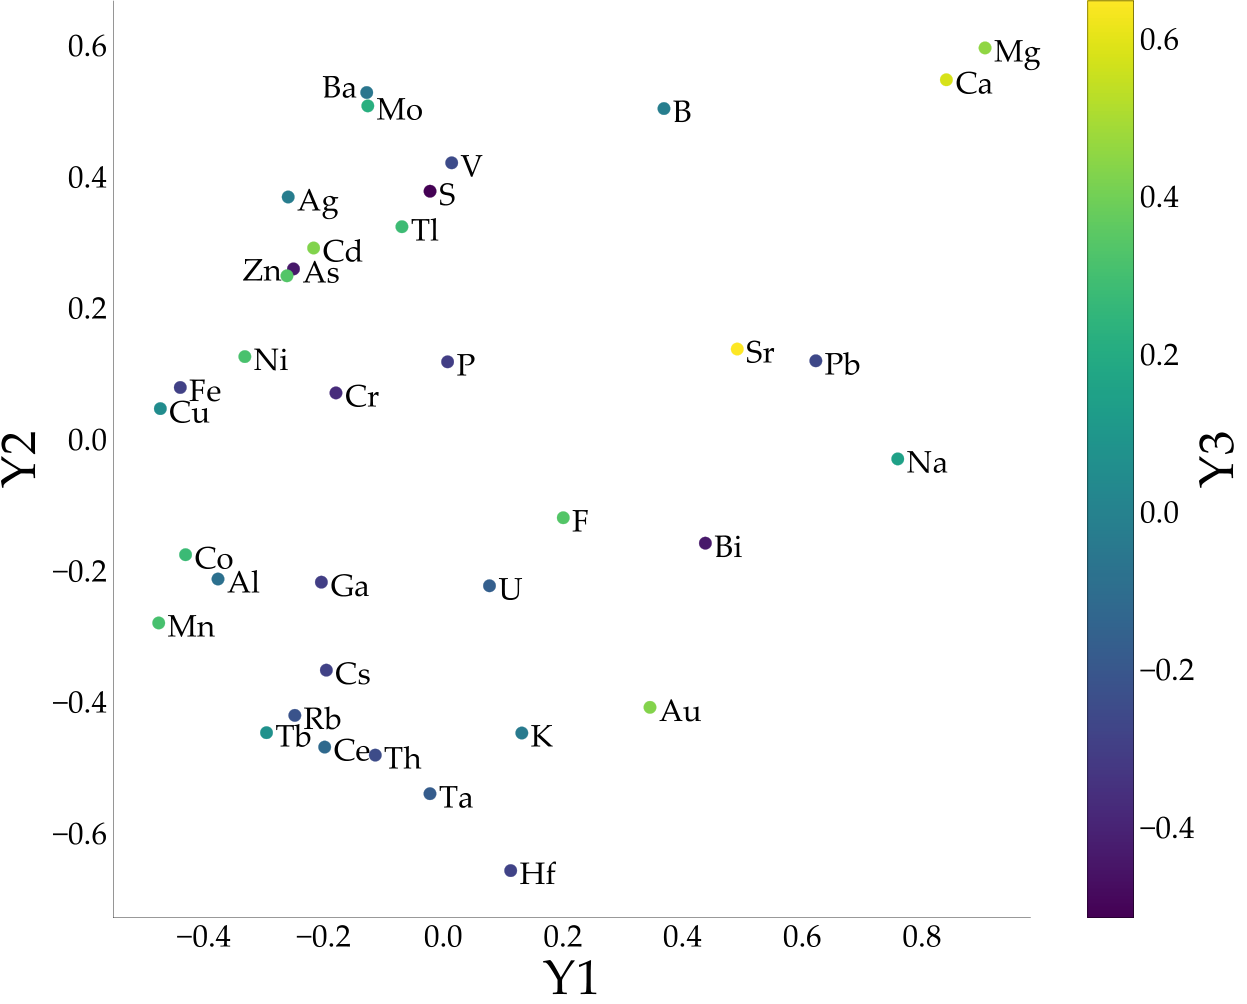
\includegraphics[scale=0.25]{gambar/MD}
          \caption{scatter plot multidimensional scaling}
          \label{md}
      \end{figure}


  \subsection{Python}
    \indent Python adalah sebuah bahasa pemrograman komputer berbasis interpreter. Python banyak dimanfaatkan diberbagai bidang. Mulai dari bidang \emph{web programming}, aplikasi desktop, \emph{backend programming} sampai dengan komputasi saintifik dan \emph{machine learning}. Python memiliki keunggulan yaitu syntax yang sederhana dan mudah dimengerti. Sehingga orang awam yang sebelumnya melakukan pemrograman komputer sangat disarankan menggunakan python untuk belajar karena mudah untuk dimengerti dan diaplikasikan.\\
    \indent keunggulan lain dari python adalah python memiliki fleksibilitas untuk menggunakan \emph{package} yang dapat memudahkan pengguna. Ini menjadi daya tarik utama untuk pengguna menggunakan python karena mereka tidak perlu menulis kode benar-benar dari nol. Mereka hanya perlu memanggil fungsi yang diinginkan dari \emph{package} yang bersangkutan.\\
    \indent Semua kemudahan yang datang bersama python tidak datang tanpa kekurangan. Python memiliki kekurangan yaitu waktu untuk mengeksekusi program yang relatif lebih lama dibandingkan bahasa pemrograman dengan basis compiler. Hal ini dikarenakan python berbasis interpreter sehingga dalam proses eksekusi program berlangsung secara baris per baris. Jadi dikembalikan lagi kepada kebutuhan dari si pengguna. Apabila pengguna membutuhkan performa yang cepat tidak disarankan menggunakan python tetapi apabila pengguna akan melakukan analisis yang kompleks sangat disarankan menggunakan python. \\
    
    \begin{figure}[H]
    	\centering
    	
\includegraphics[scale=0.5]{gambar/py}
    	\caption{logo python}
    	\label{py}
    \end{figure}

% Baris ini digunakan untuk membantu dalam melakukan sitasi
% Karena diapit dengan comment, maka baris ini akan diabaikan
% oleh compiler LaTeX.
\begin{comment}
\bibliography{daftar-pustaka}
\end{comment}
